\documentclass[12pt]{standalone}
\usepackage{bm}
\usepackage{tikz}\usetikzlibrary{arrows,shapes,trees}
\begin{document}
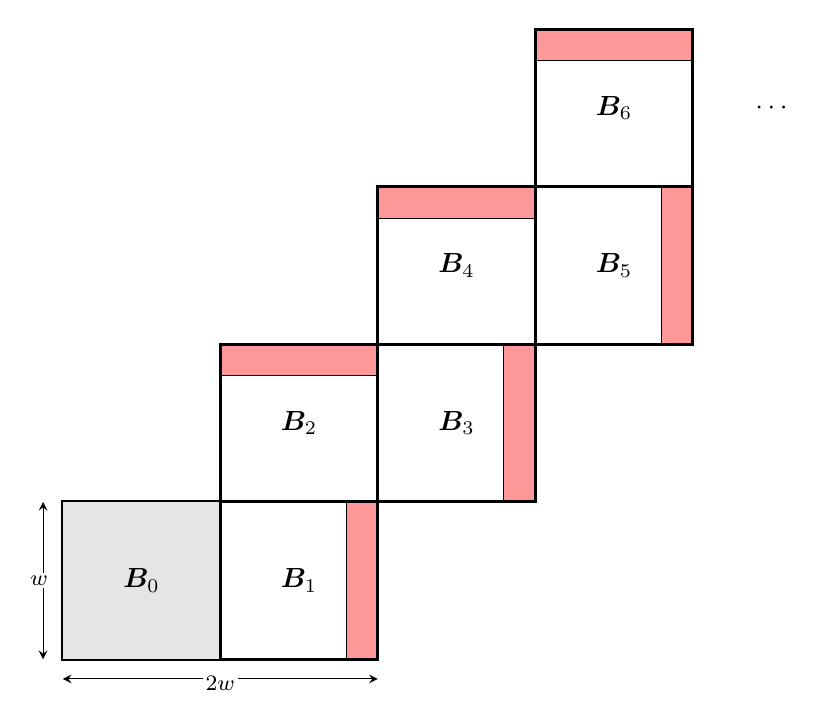
\begin{tikzpicture}[scale=1.0,>=stealth]

		\draw[arrows=<->](-0.25,0)--(-0.25,2);
		\node[fill=white,font=\footnotesize,inner sep=1pt] at (-0.3,1) {$w$};
		\draw[arrows=<->](0,-0.25)--(4,-0.25);
		\node[fill=white,font=\footnotesize,inner sep=1pt] at (2,-0.3) {$2w$};

		\draw[fill=red!40] (3.6,0) rectangle (4,2);
		\draw[fill=red!40] (2,3.6) rectangle (4,4);
		\draw[fill=red!40] (5.6,2) rectangle (6,4);
		\draw[fill=red!40] (4,5.6) rectangle (6,6);
		\draw[fill=red!40] (7.6,4) rectangle (8,6);
		\draw[fill=red!40] (6,7.6) rectangle (8,8);
		
		\foreach \i in {0,2,4, 6}
			\draw[very thick] (\i,\i) rectangle (\i+2,\i+2);
		\draw [fill=gray!20] (0,0) rectangle (2,2);
		\foreach \i in {0,2,4}
			\draw[very thick] (\i+2,\i) rectangle (\i+4,\i+2);
		\foreach \i in {0,2,4, 6}
			\node (\i) at (\i+1,\i+1) {$\bm B_\i$};
		\foreach \i in {1,3,5}
			\node (\i) at (\i+2,\i) {$\bm B_\i$};
		\node (6) at (9,7) {$\cdots$};

	\end{tikzpicture}
\end{document}
